\documentclass[11pt,answers]{exam}

% Load useful packages
% Read in necessary packages
\usepackage{import}
\usepackage{amsmath}
\usepackage{amsfonts}
\usepackage{amssymb}
\usepackage{graphicx}
\usepackage{hyperref}
\usepackage{color}
\usepackage{tikz}

% Set various options for exam package
\shadedsolutions % defines the style of the solution environment

\newcommand{\coursename}{Problem Set 9}
\newcommand{\lessonname}{}
\newcommand{\duedate}{April 26, 2016}
\newcommand{\names}{Liz Ruvolo, Meridith Richmond, Ian Gallmeister, Kevin Fortune}

\pagestyle{headandfoot}
\firstpageheader{\textbf{\large \coursename\ \lessonname}}{}{\textbf{\large Due \duedate}}
\firstpageheadrule
\runningheader{\textbf{\large \coursename\ \lessonname}}{}{\textbf{\large Due \duedate}}
\runningheadrule
\firstpagefooter{\names}{}{Page \thepage\ of \numpages}
\firstpagefootrule
\runningfooter{\names}{}{Page \thepage\ of \numpages}
\runningfootrule

\renewcommand{\theenumi}{(\textsc{\alph{enumi}})}
\renewcommand{\labelenumi}{\theenumi}
\renewcommand{\thequestion}{\arabic{question}}
\renewcommand{\questionlabel}{(\thequestion)}
\begin{document}
\begin{questions}

\addtocounter{question}{46}
\item (Gravitational equilibrium) A particle moves along a line joining two stationary masses, m1, and m2, which are separated by a fixed distance a. Let x denote the distance of the particle from m1. Find the particle’s equilibrium position. Is it stable or unstable?

\begin{solution}
The physical equation that describes this system is $\ddot{x} = \frac{Gm_2}{(x-a)^2} - \frac{Gm_1}{x^2}$ (This is given earlier in the problem). To find the equilibrium points, we need to find the points where $\ddot{x} = 0$.

$$0 = \frac{Gm_2}{(x-a)^2} - \frac{Gm_1}{x^2}$$

$$\frac{m_2x^2}{m_1} = (x-a)^2$$

This equation is quadratic and will have two solutions. This means there are two equilibrium points.

$$x_1 = \frac{a*(-m_1) -a*\sqrt[]{m_2}\sqrt[]{m_1}}{m_2-m_1}$$

$$x_2 = \frac{a*(-m_1) +a*\sqrt[]{m_2}\sqrt[]{m_1}}{m_2-m_1}$$

In this problem, the particle must be on the line between the two masses, so x cannot be negative. Therefore, we may toss the $x_1$ solution because it will be negative for all positive values $m_1,m_2, and a$.

To investigate the stability of the equilbrium point, I will use this system of equations:

$$\dot{x} = y = f(x)$$
$$\dot{y} = \frac{Gm_2}{(x-a)^2} - \frac{Gm_1}{x^2} = g(x)$$

The general Jacobian of this system is

$$\begin{pmatrix}
f_x & f_y\\ 
g_x & g_y
\end{pmatrix}$$

We cannot know what $f_x$ is without knowing $\dot{x}$. We know that $f_y$ equals one because it is the partial derivative of itself. We can solve for $g_x$. $g_y$ equals 0 because we know that $\ddot{x}$ does not contain y. This information gives the Jacobian matrix

$$\begin{pmatrix}
f_x & 1\\ 
g_x & 0
\end{pmatrix}$$

The determinant equals $f_x$*0 - $g_x$, so if $g_x$ is positive then we know that this is a saddle point. I used woflram alpha to solve for the partial derivative $g_x$:

$$g_x = 2G*(\frac{m_2}{(a-x)^3} +\frac{m_1}{x^3})$$

Remember that we are only looking for positivity. We know that x is positive because it must be on the line between the two planets. We also know that a is positive AND bigger than x by definition because it is the distance between the two planets. Therefore, every term in $g_X$ is positive, so the whole thing is positive.

The determinant is negative because $g_x$ is positive. Therefore, according the the classification system in Strogratz, the fixed point is a saddle point, meaning that it is unstable.

\end{solution}

\item Strogatz 6.4.2 Consider the follow "rabbit vs. sheep" problem, where $x,y \geq 0$. Find the fixed points, investigate their stability, draw nullclines, and sketch plausible phase portraits. Indicate the basins of attraction of any stable fixed points. 
\begin{equation}
\dot{x} = x(3-2x-y)
\end{equation}
\begin{equation}
\dot{y} = y(2-x-y)
\end{equation}

\begin{solution} \\ (i) First we find the fixed points by finding all points on the $xy$ plane where $\dot{x}$ and $\dot{y}$ are both equal to zero. \\
The most obvious point where this happens is $(0,0)$. \\
Next, we evaluate $\dot{x} = 0$ and $\dot{y} = 0$ when $y = 0$ and find that if $y = 0$, $\dot{x} = 0$ and $\dot{y} = 0$ when $x = 3/2$. \\
Next, we evaluate $\dot{x} = 0$ and $\dot{y} = 0$ when $x = 0$ and find that if $x = 0$, $\dot{x} = 0$ and $\dot{y} = 0$ when $y = 2$. \\
Lastly we set $\dot{x}$ and $\dot{y}$ equal to zero and solve for $x$ and $y$ and find that our last fixed point is $(1,1)$, per the work below. 
Starting with $\dot{x} =  0$,
\begin{equation}
3x-2x^{2}-xy = 0
\end{equation}
\begin{equation}
3x-2x^{2} = xy
\end{equation}
\begin{equation}
3 - 2x = y
\end{equation}
Now looking at $\dot{y} = 0$,
\begin{equation}
2y - xy - y^{2} = 0
\end{equation}
\begin{equation}
2y - y^{2} = xy
\end{equation}
\begin{equation}
2 - y = x
\end{equation}
Plugging our value for $x$ into our equation for $y$,
\begin{equation}
3 - 2 (2-y) = y 
\end{equation}
\begin{equation}
3 - 4 + 2y = y 
\end{equation}
\begin{equation}
-1 = y - 2y 
\end{equation}
\begin{equation}
-1 = -1y 
\end{equation}
\begin{equation}
y = 1, x = 1 
\end{equation}

So our fixed points are $(0,0)$, $(3/2, 0)$, $(0,2)$, and $(1,1)$. \\
(ii) To investigate the stability of these fixed points, we find the general Jacobian matrix and then evaluate it at each of the fixed points. In this way we are linearizing this non-linear system of equations to find an accurate approximation of its behavior at each of the fixed points. We can then generalize this into a picture of the system's dynamics in the form of a phase portrait. \\
If we say that $\dot{x} = f$ and $\dot{y} = g$, then the Jacobian matrix is 
\begin{equation} J_{general} =
\begin{pmatrix}
f_{x} & f_{y}\\ 
g_{x} & g_{g}
\end{pmatrix}
\end{equation}
or, in other words, the derivative of each of the equations governing our system with respect to one variable and then the other. \\ 
Here, the general Jacobian is 
\begin{equation}J = 
\begin{pmatrix}
3-4x-y & -x\\ 
-y & 2-x-2y
\end{pmatrix}.
\end{equation}
At $(0,0)$,  
\begin{equation}J_{(0,0)} = 
\begin{pmatrix}
3 & 0\\ 
0 & 2
\end{pmatrix}
\end{equation}
and the eigenvectors and eigenvalues of this linear approximation of the system are
\begin{equation}
\lambda_{1} = 3, 
\mathbf{v_{1}} = \begin{pmatrix}
 1\\ 
 0
\end{pmatrix},
\lambda_{2} = 2,
\mathbf{v_{2}} = \begin{pmatrix}
 0\\ 
 1
\end{pmatrix}. 
\end{equation}
This means that at $(0,0)$, this system has an unstable node, with exponential growth along the axes spanned by the eigenvectors. Near $(0,0)$, the trajectories will be tangential to the direction of the "slow" eigenvector with the lower rate of exponential growth, $\mathbf{v_{2}}$, which spans the $y$ axis.  \\

At $(3/2,0)$,  
\begin{equation}J_{(3/2,0)} = 
\begin{pmatrix}
-3 & -3/2\\ 
0 & 1/2
\end{pmatrix}, \lambda_{1} = -3, 
\mathbf{v_{1}} = \begin{pmatrix}
 1\\ 
 0
\end{pmatrix},
\lambda_{2} = 1/2,
\mathbf{v_{2}} = \begin{pmatrix}
 - 0.428571\\ 
 1
\end{pmatrix}.
\end{equation}
This means that at $(3/2,0)$ there is a saddle point, with one axis of exponential decay and one axes of exponential growth. \\

At $(0,2)$,  
\begin{equation}J_{(0,2)} = 
\begin{pmatrix}
1 & 0\\ 
-2 & -2
\end{pmatrix}, \lambda_{1} = -2, 
\mathbf{v_{1}} = \begin{pmatrix}
 0\\ 
 1
\end{pmatrix},
\lambda_{2} = 1,
\mathbf{v_{2}} = \begin{pmatrix}
 - 3\\ 
 2
\end{pmatrix}.
\end{equation}
This means that at $(0,2)$ there is again a saddle point, with one axis of exponential decay (the one associated with the -2 eigenvalue) and one axes of exponential growth (associated with the +1 eigenvalue). \\

At $(1,1)$,  
\begin{equation}J_{(1,1)} = 
\begin{pmatrix}
-2 & -1\\ 
-1 & -1
\end{pmatrix}, \lambda_{1} \approx -2.6, 
\mathbf{v_{1}} \approx \begin{pmatrix}
 1.6\\ 
 -0.6
\end{pmatrix},
\lambda_{2} \approx -0.38,
\mathbf{v_{2}} \approx \begin{pmatrix}
 - 0.61\\ 
 1
\end{pmatrix}.
\end{equation}
At this fixed point, we have a stable node, with exponential decay along both directions defined by the eigenvectors. \\

iii) Next, we draw the nullclines for this system, which are the trajectories where just $\dot{x} = 0$ or just $\dot{y} = 0$. Nullclines intersect at our fixed points.   

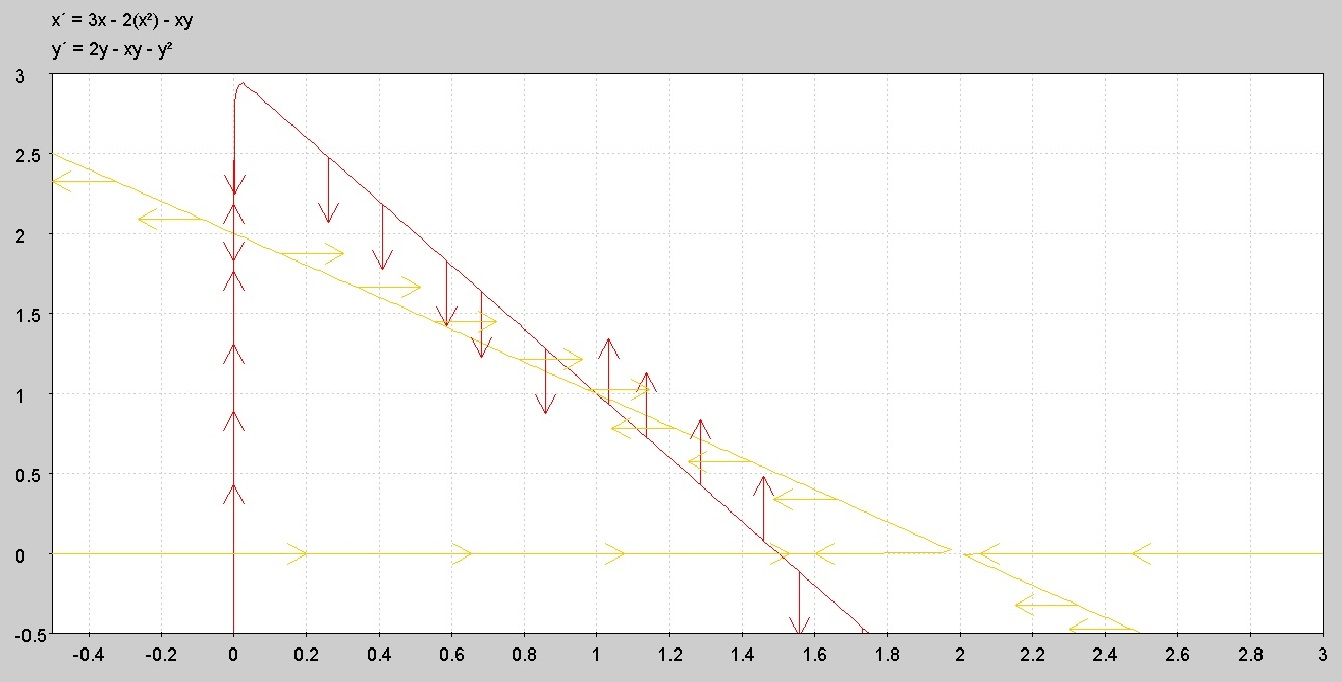
\includegraphics[width = 0.75\textwidth]{nullclines160425_a} \\

iv) Now we have more than enough information to plot a phase portrait. \\
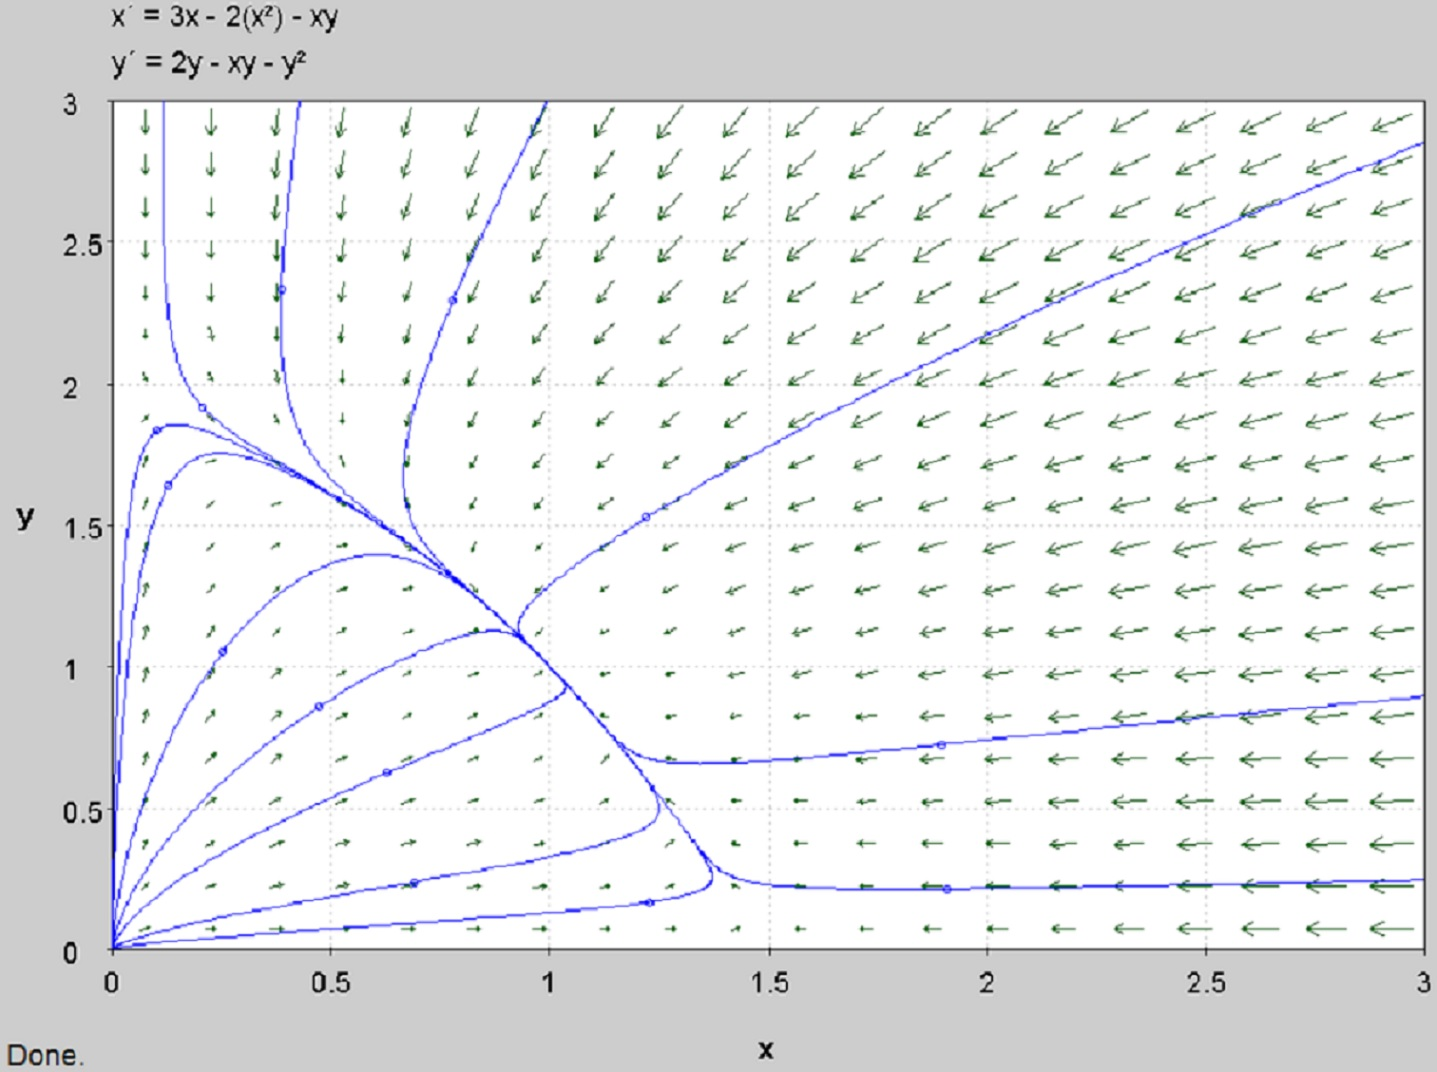
\includegraphics[width = 0.75\textwidth]{phaseportrait}\\
In terms of basins of attraction, since every logical (non-negative number of rabbits or sheep) initial condition eventually approaches our one stable node, the entire 1st quadrant is the basin of attraction for the stable fixed point at $(1,1)$. 
\end{solution}

\item (6.4.9) The ``Keynsian Cross'', a simple model of a national economy is given by
\begin{align*}
\dot{I} &= I - \alpha C, I \geq 0 \hbox{ is national income } \\
\dot{C} &= \beta( I - C - G ), C \geq 0 \hbox{ is consumer spending }
\end{align*}
and $G \geq 0$ is government spending.  $1 < \alpha < \infty, ~ 1 \leq \beta < \infty$.
\begin{enumerate}
\item Show that if $G$ is constant, there is a fixed point in the model and thus and equilibrium state in the economy.  Classify this fixed point as a function of $\alpha$ and $\beta$.  In the limiting case where $\beta = 1$, show that the economy is predicted to oscillate.
\item Next assume $G = G_0 + kI, ~ k > 0$.  Determine under which conditions there is an economically sensible equilibrium, meaning one where $I, C \geq 0$.  Show that there is a $k_c$ for which if $k > k_c$, the equilibrium case ceases to exist.  How does this economy behave when $k > k_c$?
\item Now suppose $G = G_0 + kI^2$.  Show the system can have zero, one, or two equilibrium points where $C, I \geq 0$, depending on $G_0$.  Discuss the implications for the government by interpreting the phase portraits.
\end{enumerate}

\begin{solution}
\\ \textsc{(a)} By setting $\dot{I} ~ \& ~ \dot{C} = 0$, we find that $I = \alpha C$ (and this applies to all cases).  Now, we can substitute our new value for $I$ into the equation for $\dot{C}$ to find that $\displaystyle C = \frac{G}{\alpha - 1} \hbox{ and } I = \frac{\alpha G}{\alpha - 1}$.  With our two values, we can take a look at the Jacobian evaluated at the fixed point and find that we only need the coordinates to show that the fixed point will be in the first quadrant. (It is, $\alpha > 1$ so $\alpha - 1 > 0$, and $G \geq 0$, so every piece is positive.)  The jacobian is:
\[
\left(\begin{array}{cc} 1 & -\alpha \\ \beta & -\beta \end{array}\right) \Rightarrow \begin{array}{c} \Delta = \beta(\alpha - 1) \geq 0 \\ \tau = 1 - \beta < 0 \end{array}
\]
From what we know already, we can guarantee that the fixed point is stable, but whether it is a node or spiral depends on whether $\tau^2 - 4\Delta > 0$ or not.  Above zero, and it's a node.  Less than and it's a spiral.  Simplified out, that becomes a question of whether $1 + \beta^2 + (2 - 4\alpha)\beta > 0$ or not.  We know that $1 + \beta^2$ is unquestionably positive, so we need $(2 - 4\alpha)\beta < -1 - \beta^2$ to make this a spiral.  Some manipulation leads us to $\alpha > \frac{1}{2} + \frac{\beta}{4} + \frac{1}{4\beta}$ to get a spiral.  Anything less than that gives a node.  Now, the limiting case $\beta = 1$ gives us $\tau = 0$ and $\Delta = \alpha - 1$  Here, we have a center since the determinant is positive and the trace is zero, so we don't need to worry about $\tau^2 - 4\Delta$.  This means that if the economy is at some point not at the fixed point, the phase portrait carves out a cycle about the center, oscillating all over the place. (Well, not quite, but that's ok.) 

\vspace{1em}

\textsc{(b)} Here, we have the same value of $I$ for $\dot{I} = 0$, and after substituting that and $G_0 + kI$ for $G$ into $\dot{C}$, we get that $\dot{C} = \beta((\alpha - 1 - \alpha k)C - G_0)$ so $C = \frac{G_0}{\alpha - \alpha k - 1}$.  In order to make sure this value of $C$ stays positive, we need $\alpha > \alpha k - 1$, which gives us our $\displaystyle k_c = 1 - \frac{1}{\alpha}$.  Once again, we don't need the fixed point to find the Jacobian which is:
\[
\left(\begin{array}{cc} 1 & -\alpha \\ \beta(1 - k) & -\beta \end{array}\right) \Rightarrow \begin{array}{c} \tau = 1 - \beta \\ \Delta = \beta(\alpha(1 - k) - 1) \end{array}
\]
It's interesting to note that the denominator of $C$ is the determinant of the Jacobian which means that we need to keep $C$ positive to keep the function stable.  This would be a condition for an economically sensible equilibrium to make sure the equilibrium exists AND that $C \geq 0$

\vspace{1em}

\textsc{(c)} Once again $I = \alpha C$ for $\dot{I} = 0$.  Substituting for $I$ and $G$ gives $\dot{C} = \beta(\alpha^2 k C^2 + (\alpha - 1)C + G_0)$, so this is a quadratic and 
\[
C = \frac{(\alpha - 1) \pm \sqrt{(\alpha ^2 - 2\alpha + 1) + 4G_0\alpha^2 k}}{2\alpha^2 k} = \frac{(\alpha - 1) \pm \sqrt{\alpha^2 (1 + 4G_0k) - 2\alpha + 1}}{2\alpha^2 k}
\]
Because this is a quadratic, there are two solutions, but the value of $G_0$ can make the square root negative, in which case the roots are all messed up.  If $G_0 = 0$, then there are two roots ($C = 0, 2\alpha - 2$, both positive), and a larger $G$ makes the value of the square root larger, so there will be one root with positive $C$ and one with negative.

\end{solution}
\end{questions}

\end{document}